%%%%%%%%%%%%%%%%%%%%%%%%%%%%%%%%%%%%%%%%%
% 
% LaTeX Template
% Version 3.1 (25/3/14)
%
%%%%%%%%%%%%%%%%%%%%%%%%%%%%%%%%%%%%%%%%%

%----------------------------------------------------------------------------------------
%	PACKAGES AND DOCUMENT CONFIGURATIONS
%----------------------------------------------------------------------------------------

\documentclass[12pt, a4 paper]{article}

\usepackage{tikz}
%\usepackage[top=2cm, bottom=2cm, outer=0cm, inner=0cm]{geometry}
\usepackage{graphicx} % Required for the inclusion of images
\usepackage{multicol} % Required for multicolumns
\usepackage{setspace} % Required for line spacing
\setlength\parindent{0pt} % Removes all indentation from paragraphs
\setlength{\columnseprule}{0.4pt} % Adds vertical line between multicolumns
\usepackage{multirow} % Required for multirows
\usepackage{booktabs} % For prettier tables
\usepackage{ragged2e}
\usepackage{xcolor}
%\usepackage{tabularx}
%\renewcommand{\rmdefault}{ptm}

%\usepackage{helvet}

\usepackage{times} % Uncomment to use the Times New Roman font

%----------------------------------------------------------------------------------------
%	DOCUMENT INFORMATION
%----------------------------------------------------------------------------------------

\begin{document}

\tikz[remember picture,overlay] \node[inner sep=0pt] at (current page.center){
\includegraphics[width=\paperwidth,height=\paperheight]{image1.jpg}};

\clearpage

%\font\myfont=cmr12 at 35pt
%\title{\myfont  Event Name} % Write Event name here
%\author{}
%\date{\vspace{-10ex}}

%\maketitle % Insert the title, author and date
\setstretch{1}

\tikz[remember picture,overlay] \node[opacity=0.8,inner sep=0pt] at (current page.center){
\includegraphics[width=\paperwidth,height=\paperheight]{Border48-A4--Arvin61r58.png}};
%\tikz[remember picture,overlay] \node[opacity=0.5,inner sep=0pt] at (current page.center){\includegraphics[width=\paperwidth,height=\paperheight]{color-2174049__340.png}};

\begin{center}
\Huge \bfseries \ttfamily PROJECT EXHIBITION
\end{center}

\begin{center}
\large Technical Exhibition in the college
\end{center}

\begin{center}
\begin{multicols}{2}
\begin{tabular}{l r}
Date: & 08/04/2019\\ % Date the event was held
Time: & 2 P.M onwards \\ % Time of event 
\end{tabular}

\columnbreak

\begin{tabular}{l r}
Venue: & TCC Seminar Hall \\ % Venue of event
Total Attendance: & 17 \\ % Number of participants
\end{tabular}
\end{multicols}

\begin{Large}
\begin{multicols}{2}
\justify
GNDEC organized an event "PROJECT EXHIBITION”, a technical event on 08.04.2019. Single or team, both entries were allowed.
\columnbreak


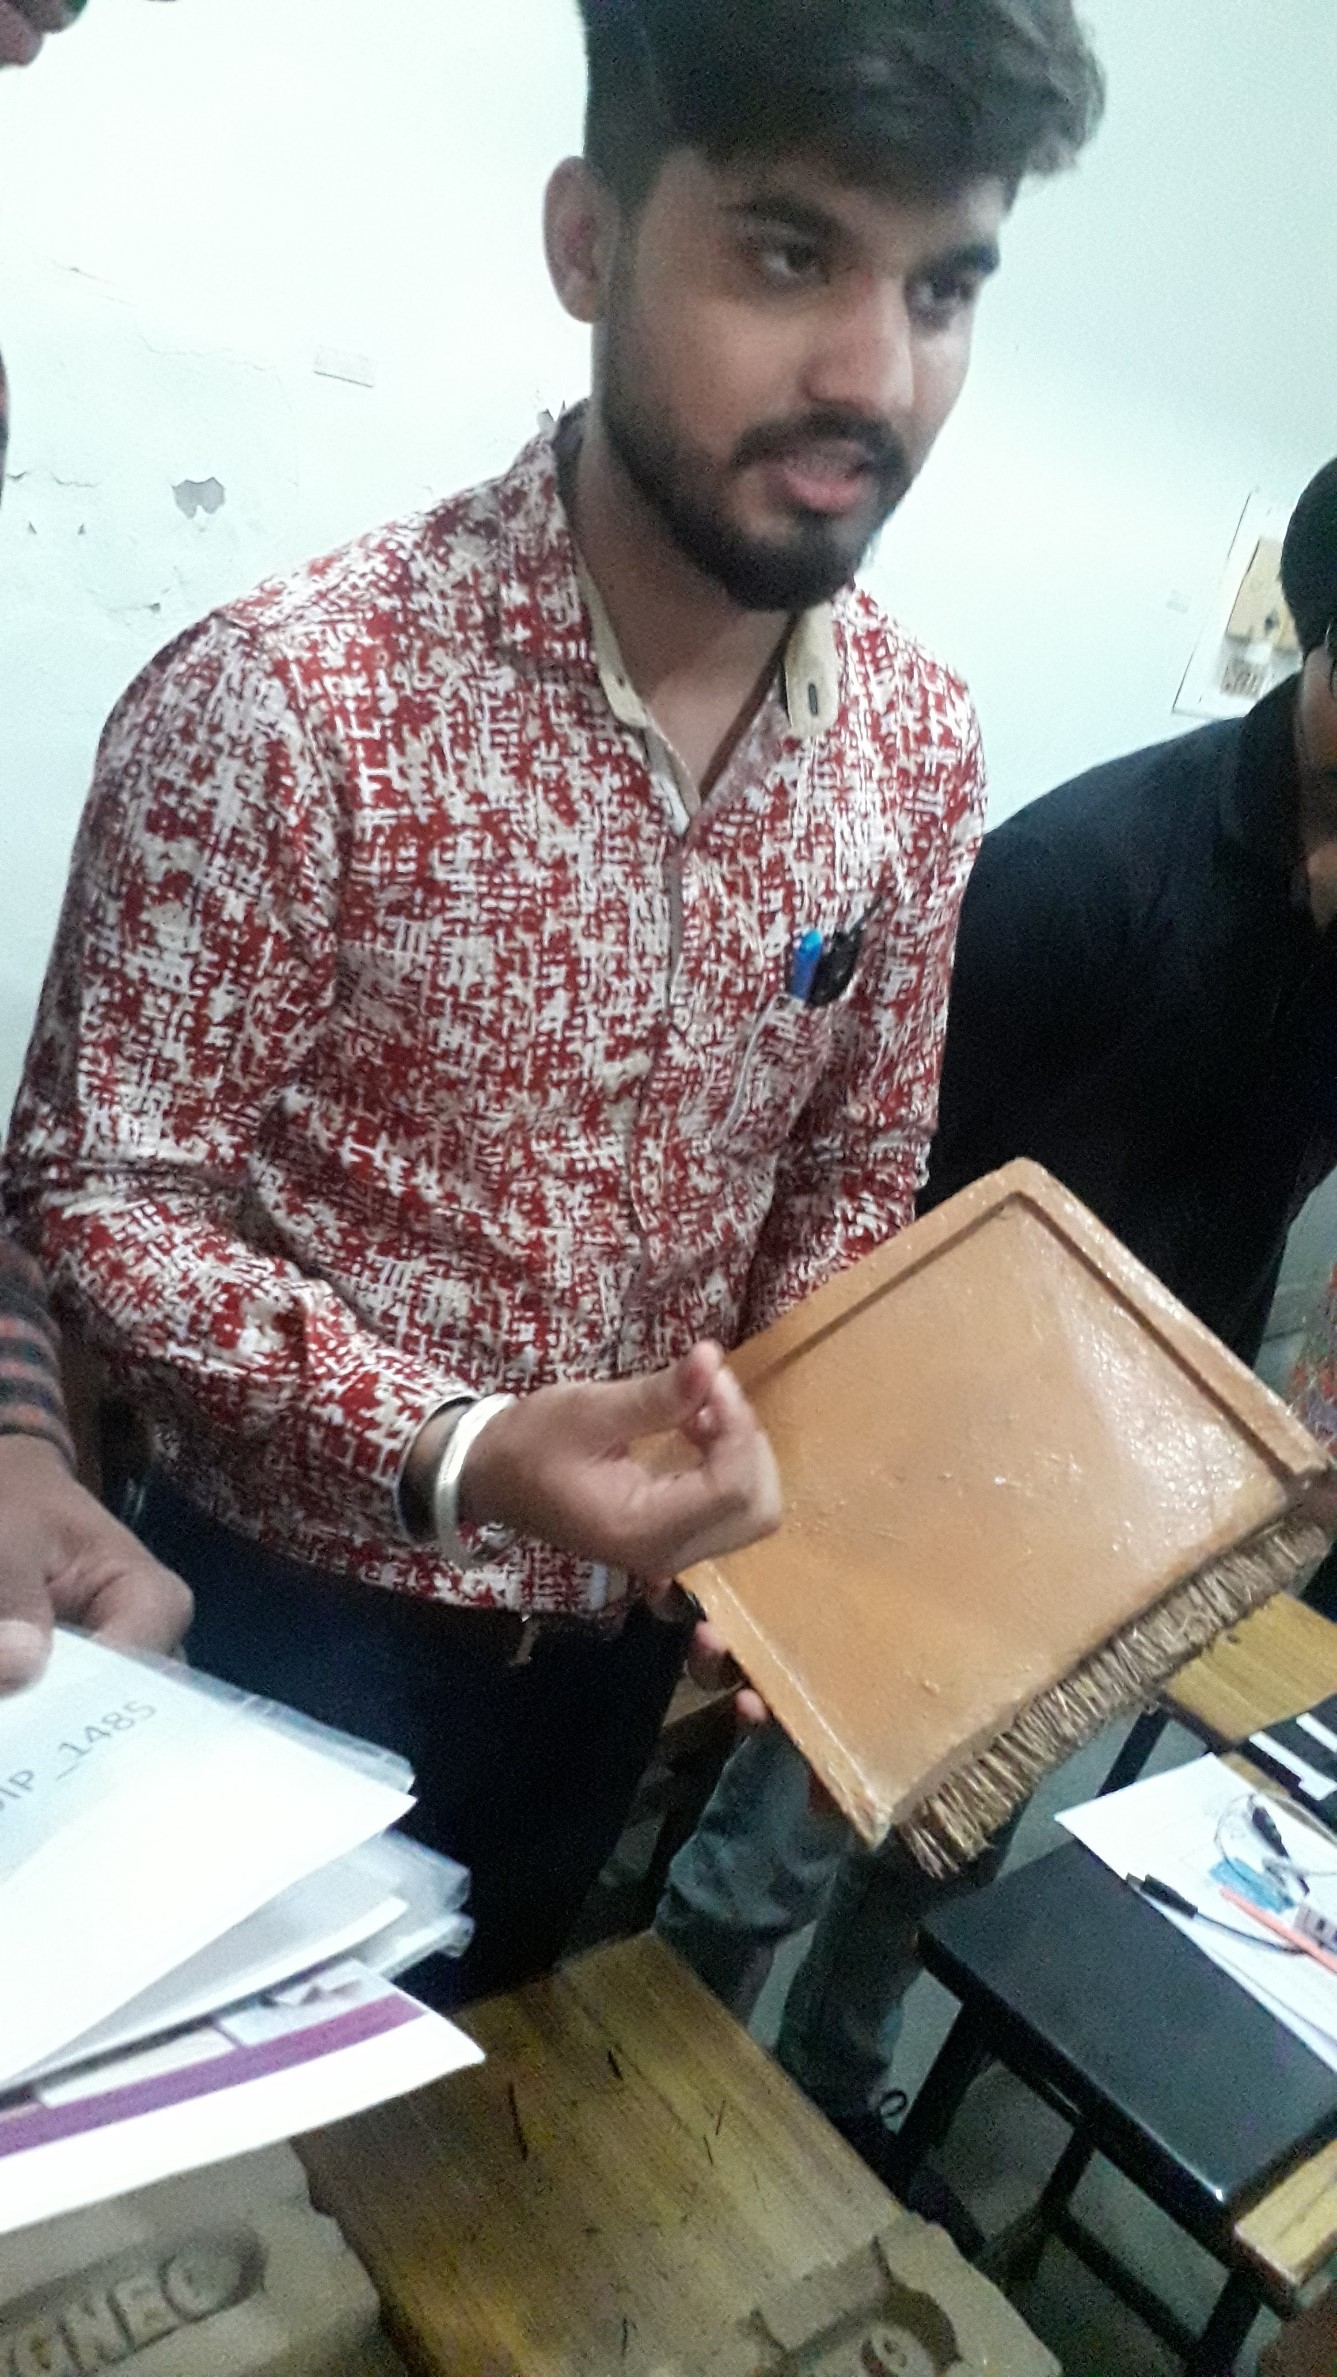
\includegraphics[width=\linewidth,height=6cm]{image8.jpeg}
  %\caption{A boat.}
  %\label{fig:boat1}
\end{multicols}

\begin{multicols}{2}

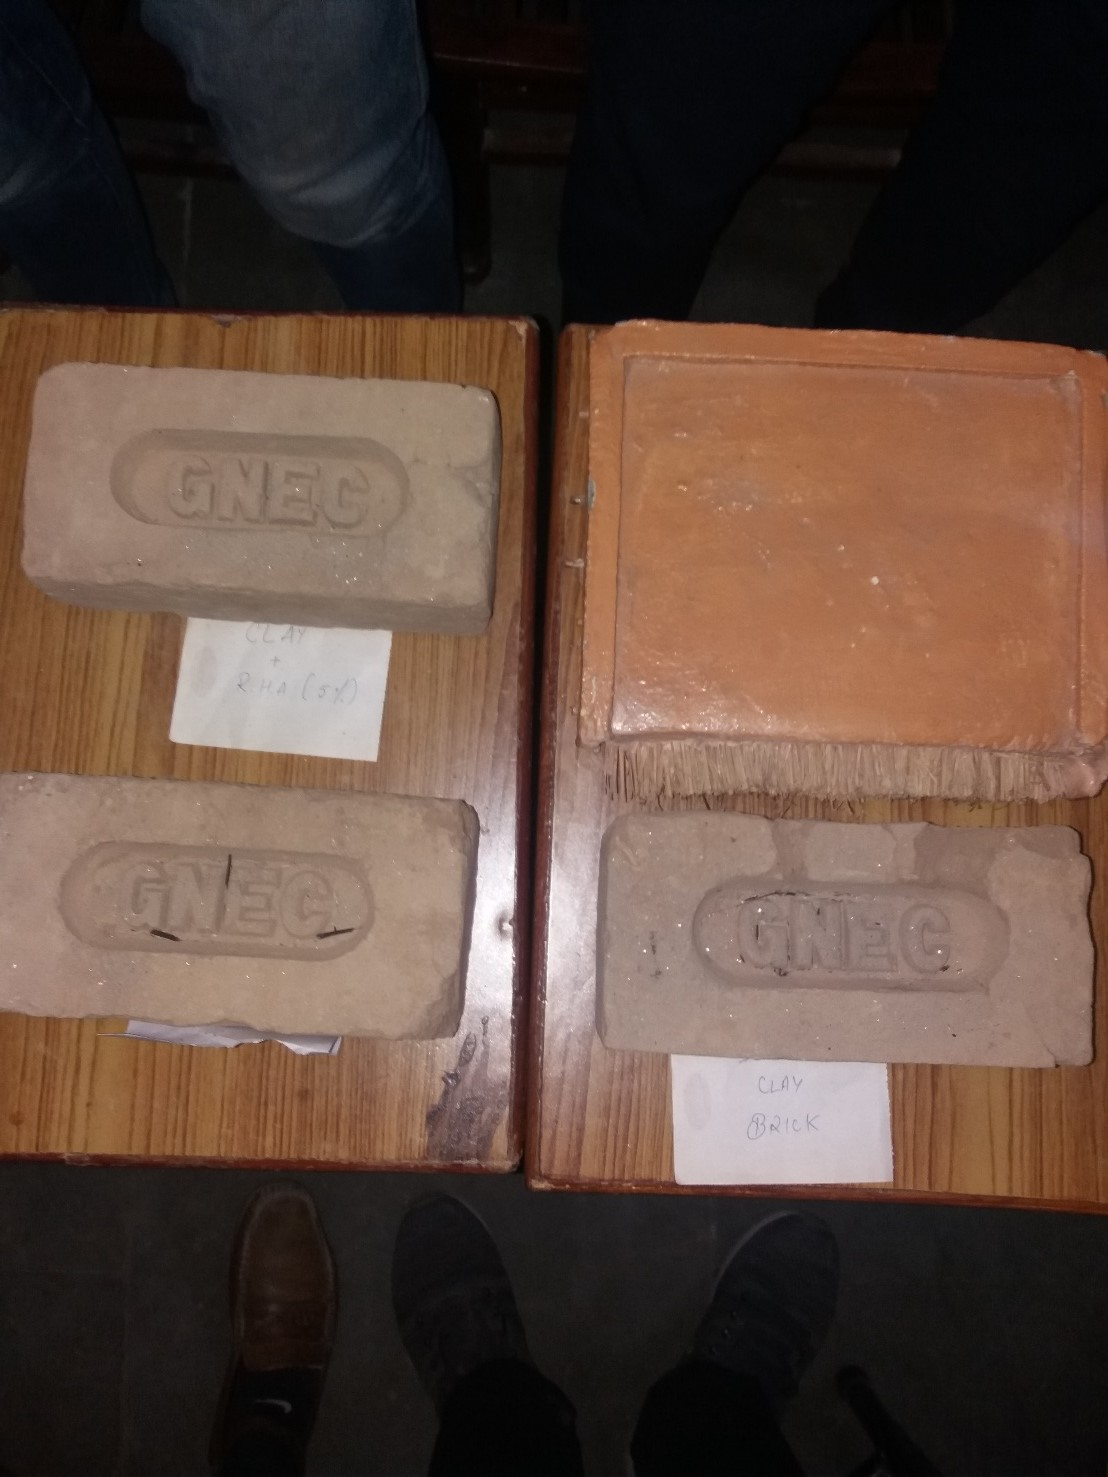
\includegraphics[width=\linewidth,height=6cm]{image7.jpeg}

\columnbreak
\justify
The motive of the event was to bring out the innovative ideas and technical skills of the students. In this event, students had to explain 
\end{multicols}

\newpage 

\tikz[remember picture,overlay] \node[opacity=0.8,inner sep=0pt] at (current page.center){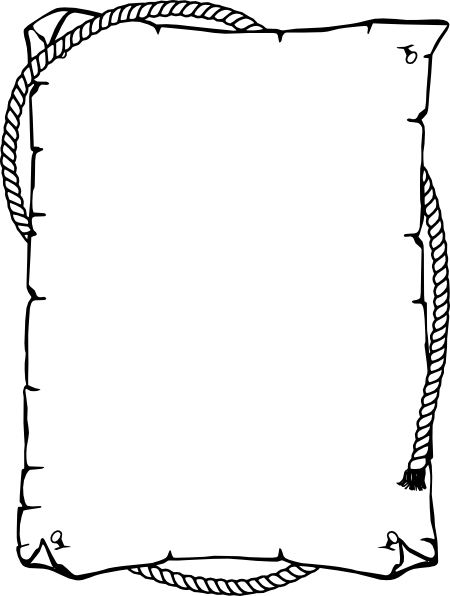
\includegraphics[width=\paperwidth,height=\paperheight]{5TRrp44jc.png}};
%\tikz[remember picture,overlay] \node[opacity=0.8,inner sep=0pt] at (current page.center){\includegraphics[width=\paperwidth,height=\paperheight]{md_5b0912b7c0870.png}};

\begin{multicols}{2}
\justify
their project and the innovative ideas that they had implemented in their projects. The judgment was based upon innovation, description, and presentation.
\columnbreak
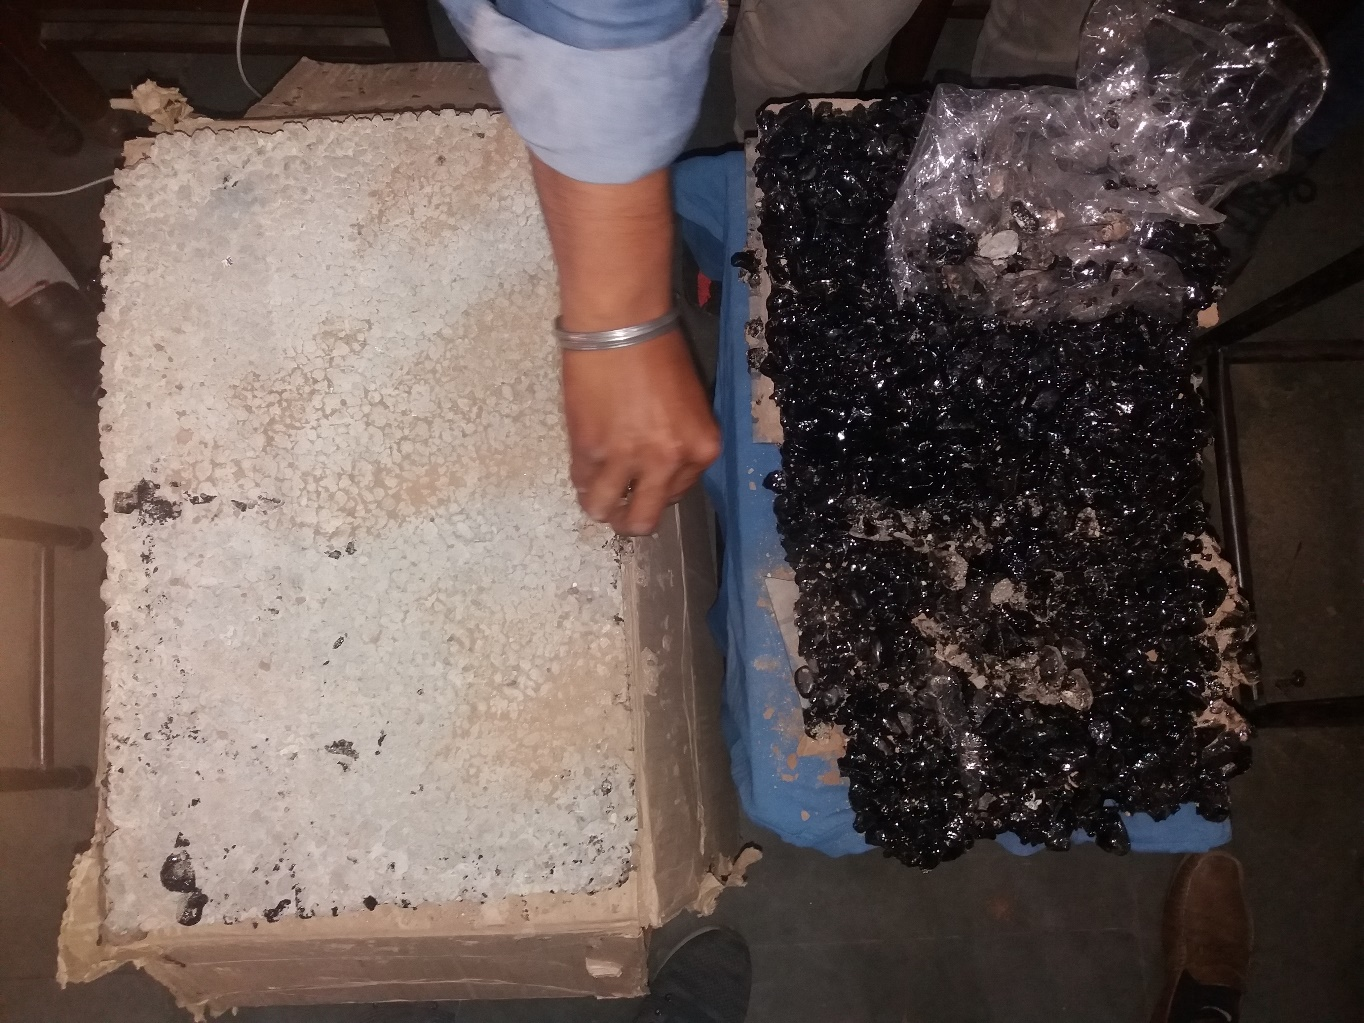
\includegraphics[width=\linewidth]{image4.jpeg}
  
\end{multicols}

\begin{multicols}{2}
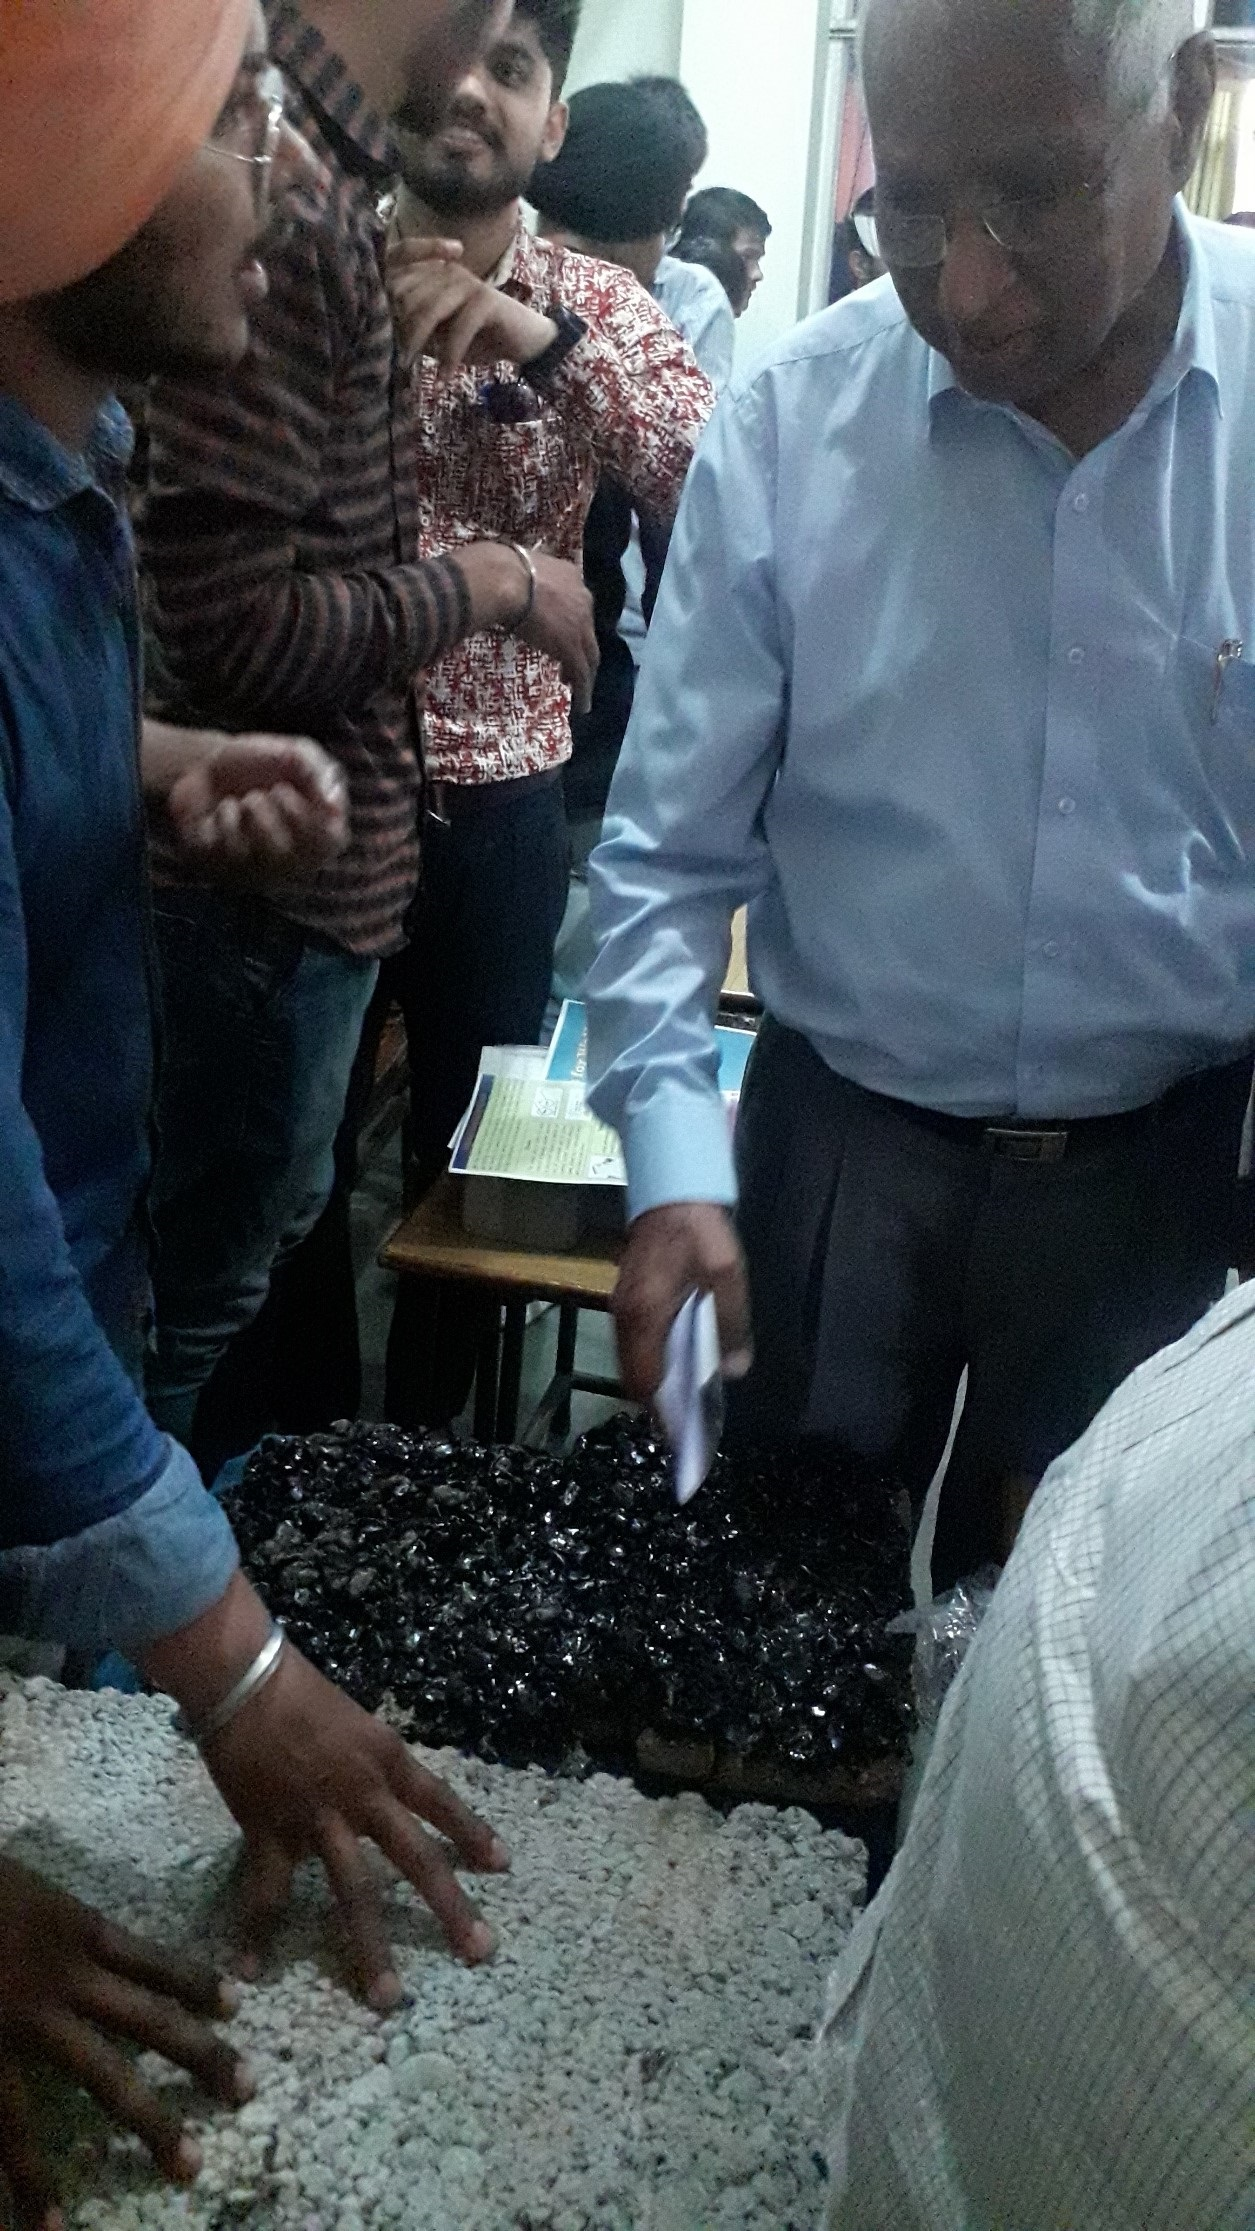
\includegraphics[width=\linewidth,height=6cm]{image9.jpeg}

\columnbreak
\justify
The event took place 
outside TCC Seminar Cell at 02:00 P.M around 17 
students participated in the event.
  
\end{multicols} 

\begin{multicols}{2}
\justify
The name of the participants, organizing team and the winners are mentioned below.

\columnbreak

\includegraphics[width=\linewidth]{image6.jpeg}
  
\end{multicols} 

%\begin{multicols}{2}
%\includegraphics[width=\linewidth]{placeholder.jpg}

%\columnbreak
%Some paragraph
  
%\end{multicols} 

\end{Large} 
\end{center}

\newpage 

\tikz[remember picture,overlay] \node[opacity=0.8, inner sep=0pt] at (current page.center){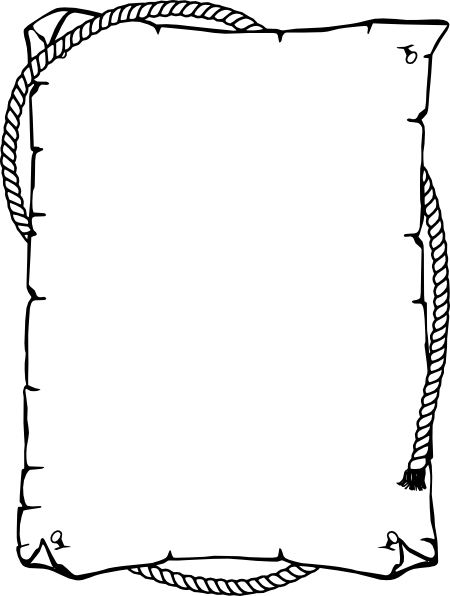
\includegraphics[width=\paperwidth,height=\paperheight]{5TRrp44jc.png}};
%\tikz[remember picture,overlay] \node[opacity=0.8,inner sep=0pt] at (current page.center){\includegraphics[width=\paperwidth,height=\paperheight]{md_5b0912b7c0870.png}};

\begin{center}
\Huge Pictures Section

\medskip

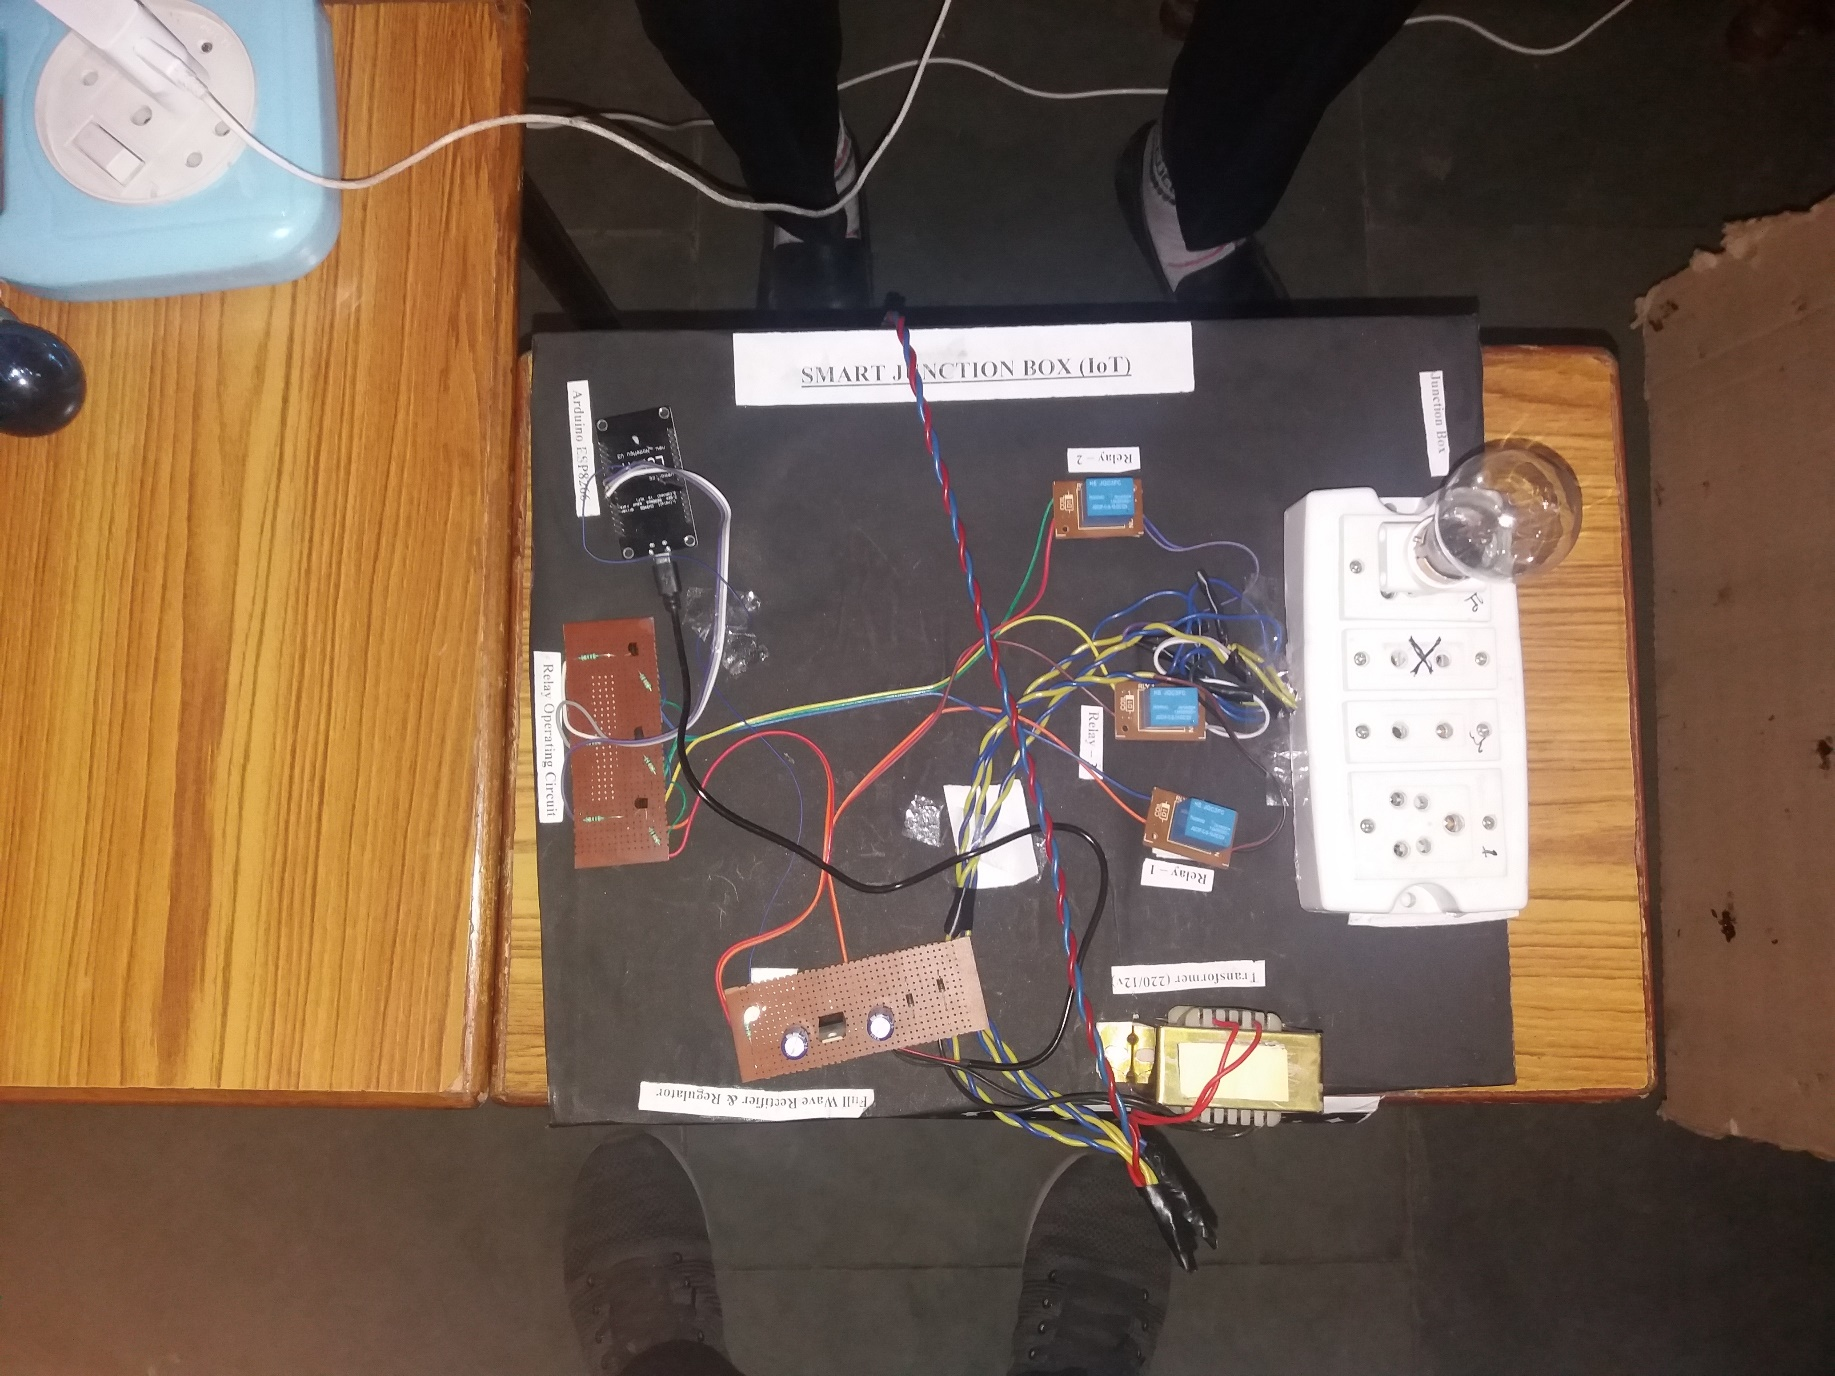
\includegraphics[height=6cm]{image2.jpeg}

\medskip


\includegraphics[height=6cm]{image3.jpeg}

\medskip

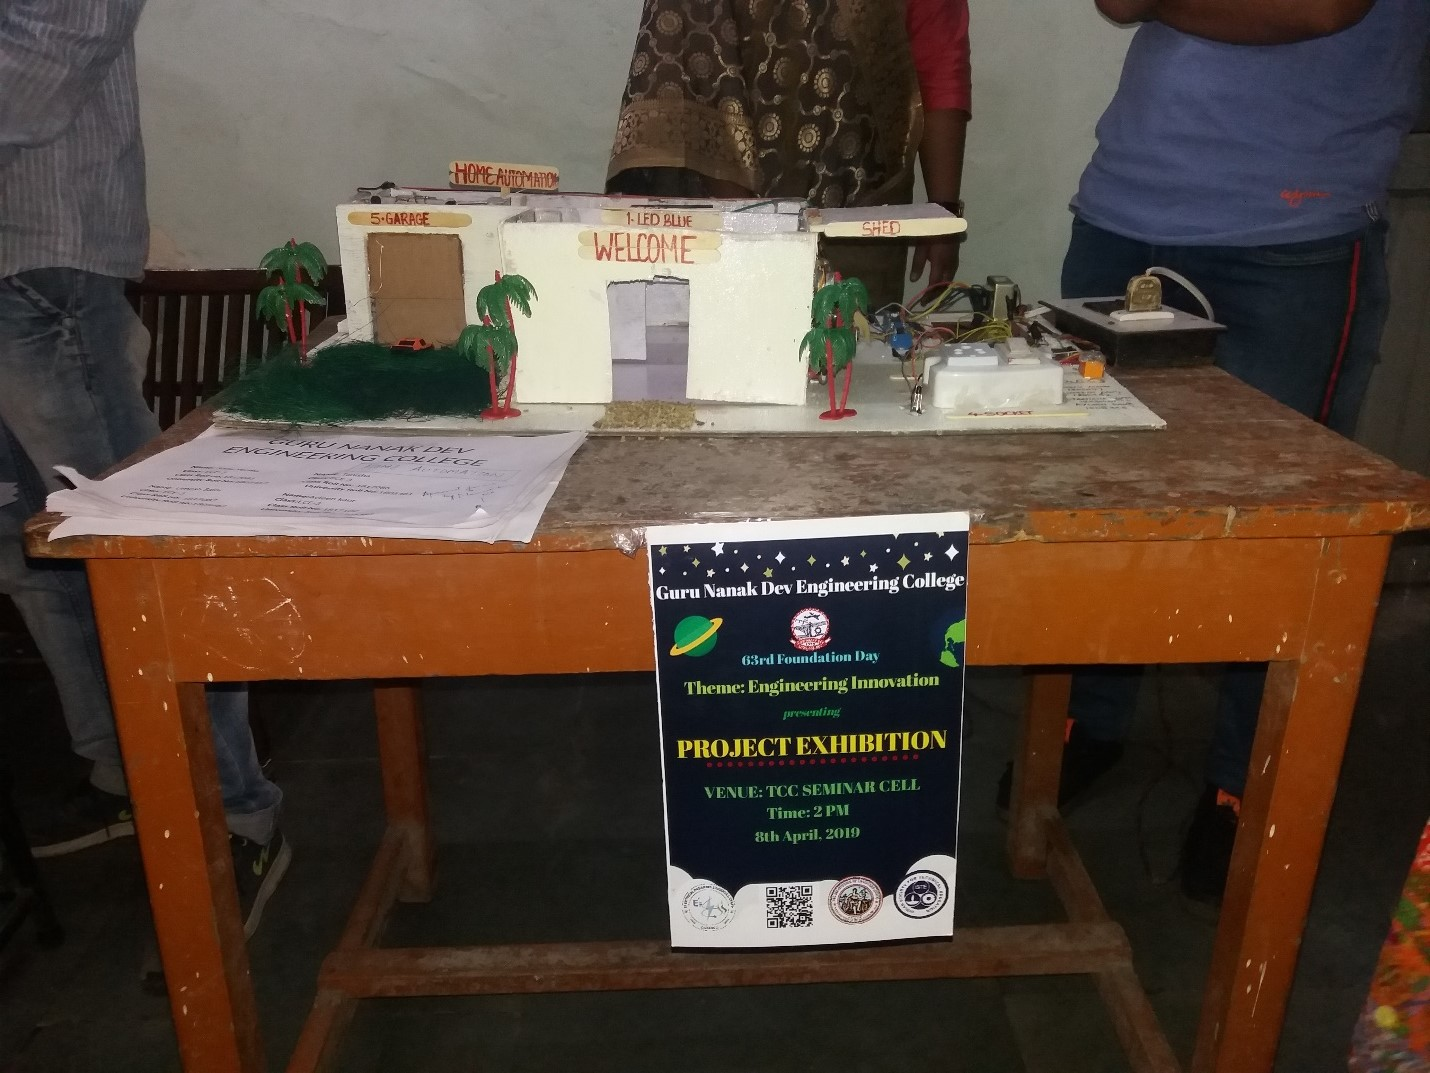
\includegraphics[height=6cm]{image5.jpeg}

\end{center}

\newpage

\begin{center}
\huge Organisers list
\end{center}

\begin{table}[h!]
  \begin{center}
    \begin{tabular}{|c|c|c|c|c|c|} 
    \toprule % <-- Toprule here
      \textbf{S.No.} & \textbf{Name} & \textbf{Branch/Year} & \textbf{U.R.N} \\
      \midrule % <-- Midrule here
      1 & Manik Walia	     & D3 EE & 1706688 \\
      2 & Kunal Singla	     & D3 EE & 1706687 \\
      3 & Neha Dwivedi	     & D3 EE & 1706691 \\
      4 & Simran Kaur Rajpal & D3 EE & 1706694 \\
      5 & Tania Sharma	     & D3 EE & 1606909 \\
      6 & Abhishek Goyal	 & D3 EE & 1706672 \\
      7 & Gurpartap Singh	 & D3 EE & 1706680 \\
      8 & Paras Joshi	     & D2 EE & 1805362 \\
      9 & Shubham Pundhir	 & D2 EE & 1706655 \\

      \bottomrule % <-- Bottomrule here
    \end{tabular}
  \end{center}
\end{table}

\tikz[remember picture,overlay] \node[opacity=0.8,inner sep=0pt] at (current page.center){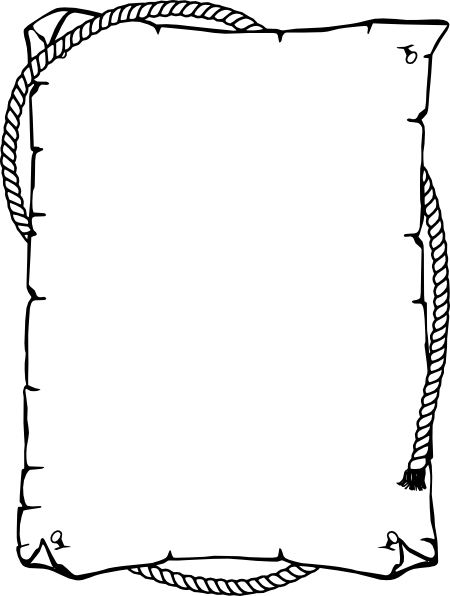
\includegraphics[width=\paperwidth,height=\paperheight]{5TRrp44jc.png}};
%\tikz[remember picture,overlay] \node[opacity=0.8,inner sep=0pt] at (current page.center){\includegraphics[width=\paperwidth,height=\paperheight]{md_5b0912b7c0870.png}};

\newpage

\begin{center}
\huge Winners List
\end{center}

\begin{table}[h!]
  \begin{center}
    \begin{tabular}{|c|c|c|c|c|c|} 
    \toprule % <-- Toprule here
      \textbf{S.No.} & \textbf{Name} & \textbf{Branch/Year} & \textbf{U.R.N} &\textbf{Position} \\
      \midrule % <-- Midrule here
       	1  & Sonu Verma	        & D1 ECE & 1805457 & \multirow{8}{*}{1st} \\
        2  & Umesh Saini	    & D1 ECE & 1805462 & \\
        3  & Tanisha Gupta	    & D1 ECE & 1805461 & \\
        4  & Avleen Kaur	    & D1 ECE & 1805383 & \\
        5  & Gurjant Singh	    & D4 EE	 & 1507717 & \\
        6  & Gourav Singla	    & D4 EE	 & 1507714 & \\
        7  & Gurbinder Singh	& D4 EE	 & 1507715 & \\
        8  & Agamdeep Singh	    & D4 EE	 & 1507697 & \\
        9  & Prabhudeep Singh	& D3 IT	 & 1607134 & \multirow{4}{*}{2nd} \\
        \hline
	    10 & Ravneet Singh	    & D3 CSE & 1606751 & \\
	    11 & Dheeraj Kumar	    & D1 ECE & 1805391 & \\
	    12 & Harmeet Singh	    & D1 ECE & 1805401 & \\
	    13 & Anmol Puri	        & D2 CE	 & 1819937 & \multirow{5}{*}{3rd} \\
	    \hline
		14 & Gurdeep Singh	    & D3 CE	 & 1706348 & \\
		15 & Siddharth Popli	& D3 CE	 & 1706374 & \\
		16 & Satinder Pal Singh & D3 CE	 & 1706373 & \\
		17 & Robin Singh	    & D3 CE	 & 1706371 & \\

      \bottomrule % <-- Bottomrule here
    \end{tabular}
  \end{center}
\end{table}

\tikz[remember picture,overlay] \node[opacity=0.8,inner sep=0pt] at (current page.center){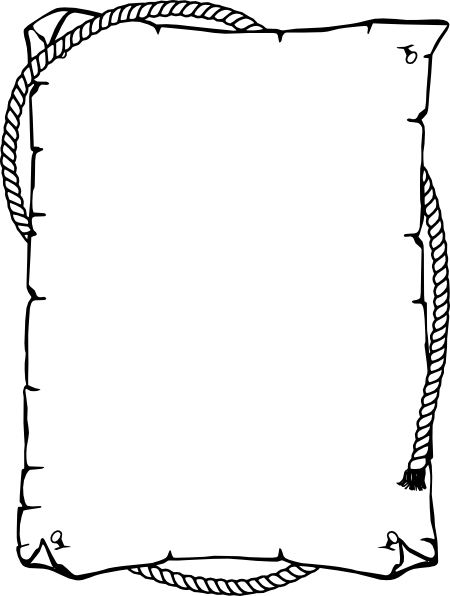
\includegraphics[width=\paperwidth,height=\paperheight]{5TRrp44jc.png}};

\newpage

\tikz[remember picture,overlay] \node[opacity=0.8,inner sep=0pt] at (current page.center){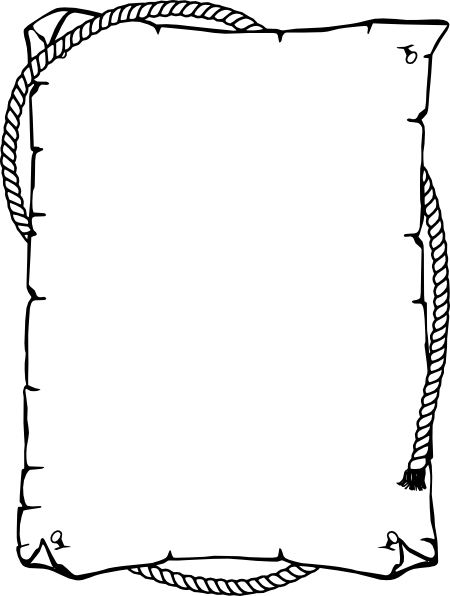
\includegraphics[width=\paperwidth,height=\paperheight]{5TRrp44jc.png}};


\begin{center}
\huge Participant list
\end{center}

\begin{table}[h!]
  \begin{center}
    \begin{tabular}{|c|c|c|c|c|c|} 
    \toprule % <-- Toprule here
      \textbf{S.No.} & \textbf{Name} & \textbf{ISTE ID} &\textbf{Year/Branch} & \textbf{URN}\\
      \midrule % <-- Midrule here
      1  & Sonu Verma	      & D1 ECE & 1805457 & 8556970889 \\
      2  & Umesh Saini	      & D1 ECE & 1805462 & 7973191593 \\
      3  & Tanisha Gupta      & D1 ECE & 1805461 & 9592578229 \\
      4  & Avleen Kaur	      & D1 ECE & 1805383 & 7973354887 \\
      5  & Dheeraj Kumar	  & D1 ECE & 1805391 & 6284501227 \\
      6  & Harmeet Singh	  & D1 ECE & 1805401 & 8168838285 \\
      7  & Gurjant Singh	  & D4 EE  & 1507717 & 7508732090 \\
      8  & Gourav Singla	  & D4 EE  & 1507714 & 9779086761 \\
      9  & Gurbinder Singh	  & D4 EE  & 1507715	          \\
      10 & Agamdeep Singh	  & D4 EE  & 1507697	          \\
      11 & Prabhudeep Singh   & D3 IT  & 1607134 & 9803794468 \\
      12 & Ravneet Singh	  & D3 CSE & 1606751 & 6280589339 \\
      13 & Anmol Puri	      & D2 CE  & 1819937 & 8360169179 \\
      14 & Gurdeep Singh	  & D3 CE  & 1706348 & 9855613690 \\
      15 & Siddharth Popli	  & D3 CE  & 1706374 & 9041842706 \\
      16 & Satinder Pal Singh & D3 CE  & 1706373 & 9781067732 \\
      17 & Robin Singh	      & D3 CE  & 1706371 & 8872647154 \\

      \bottomrule % <-- Bottomrule here
    \end{tabular}
  \end{center}
\end{table}



\end{document}